\documentclass{article}
\usepackage[utf8]{inputenc}
\usepackage{listings}
\usepackage{xcolor}
\usepackage{geometry}
\usepackage{mathtools}
\usepackage{listings}
\usepackage{hyperref}
\geometry{margin=1in}

\begin{document}
\Large{\texttt{Name: Bhargey Mehta}}

\Large{\texttt{SID : \space 201701074}}

\Large{\texttt{Info: AGT - Project - Sequential HopcroftKarp}}

\section{Algorithm}
We will be using the Hopcroft-Karp algorithm which produces a maximum matching in a bipartite graph. Note that $X$ and $Y$ are the bipartitions of the bipartite graph $G$ and $M$ is some matching of $G$. If $G$ has a perfect matching then any maximum matching is also a perfect matching.

\vspace{0.5cm}

Subroutine: BFS($X, Y, M$) \dotfill

\hspace{1cm} $G_{\mathrm{BFS}} \leftarrow$ empty graph

\hspace{1cm} visited $\leftarrow$ empty Set

\hspace{1cm} $Q \leftarrow$ empty Queue

\hspace{1cm} for each node $v$ in $B_1$

\hspace{2cm} if $v \notin M$

\hspace{3cm} enqueue $v$ in $Q$

\hspace{3cm} add $v$ to visited

\hspace{1cm} while $Q$ is NOT empty

\hspace{2cm} $v \leftarrow$ dequeue from $Q$

\hspace{2cm} if $v \in X$

\hspace{3cm} for each edge $(v, w)$ adjacent to $v$ such that $(v, w) \notin M$

\hspace{4cm} add $(v, w)$ to $G_{\mathrm{BFS}}$

\hspace{4cm} enqueue $w$ in $Q$

\hspace{4cm} add $w$ to visited

\hspace{2cm} else

\hspace{3cm} for each edge $(v, w)$ adjacent to $v$ such that $(v, w) \in M$

\hspace{4cm} add $(v, w)$ to $G_{\mathrm{BFS}}$

\hspace{4cm} enqueue $w$ in $Q$

\hspace{4cm} add $w$ to visited

\hspace{1cm} return $G_{\mathrm{BFS}}$

Subroutine: DFS($G_{\mathrm{BFS}}, M$) (wrapper function) \dotfill

\hspace{1cm} visited $\leftarrow$ empty set

\hspace{1cm} disjointPaths $\leftarrow$ empty set

\hspace{1cm} for each node $v$ in $Y$

\hspace{2cm} if $v \notin M$

\hspace{3cm} $P \leftarrow$ empty path 

\hspace{3cm} actualDFS($G_{\mathrm{BFS}}, M, v$, visited, $P$)

\hspace{3cm} add $P$ to disjointPaths if $P$ is NOT empty

\hspace{1cm} return disjointPaths

\vspace{0.5cm}

Subroutine: actualDFS($G_{\mathrm{BFS}}, M, v$, visited, $P$) \dotfill

\hspace{1cm} if $v$ in visited

\hspace{2cm} return False

\hspace{1cm} add $v$ to visited

\hspace{1cm} for all edges $(v, w)$ adjacent to $v$ in $G_{\mathrm{BFS}}$

\hspace{2cm} if ($v \in X$ and $(v,w) \notin M$) or ($v \in Y$ and $(v,w) \in M$)

\hspace{3cm} skip edge

\hspace{2cm} append $(v, w)$ to $P$

\hspace{2cm} if $w \notin M$

\hspace{3cm} add $w$ to visited

\hspace{3cm} return True

\hspace{2cm} foundPath $\leftarrow$ actualDFS($G_{\mathrm{BFS}}, M, w$, visited, $P$)

\hspace{2cm} if foundPath is True

\hspace{3cm} return True

\hspace{2cm} remove $(v, w)$ from $P$

\hspace{1cm} return False

\vspace{0.5cm}

Subroutine: HopcroftKarp($X, Y, G$) \dotfill

\hspace{1cm} if $|X|$ NOT equal $|Y|$ or $G$ is not $r-regular$

\hspace{2cm} report NO PERFECT MATCHING

\hspace{1cm} $M \leftarrow$ empty matching

\hspace{1cm} $G_{\mathrm{BFS}} \leftarrow$ BFS($X, Y, M$)

\hspace{1cm} disjointPaths $\leftarrow$ DFS($G_{\mathrm{BFS}}, M$)

\hspace{1cm} while disjointPaths is NOT empty

\hspace{2cm} augment $M$ with each $P$ in disjointPaths

\hspace{2cm} $G_{\mathrm{BFS}} \leftarrow$ BFS($X, Y, M$)

\hspace{2cm} disjointPaths $\leftarrow$ DFS($G_{\mathrm{BFS}}, M$)

\hspace{1cm} return $M$

\section{Proof of Correctness}
\subsection{Augmenting Path Lemma}
Augmenting Path Lemma: A matching $M$ of $G$ is maximum if and only if there is no augmenting path in $G$.

This lemma has been proved in the lecture, so we use it as it is.

\subsection{Disjoint Paths Lemma}
Disjoint Path Lemma: The paths returned by the DFS subroutine are vertex disjoint and are augmenting paths of $M$ wrt $G$.

\begin{figure}[!h]
    \centering
    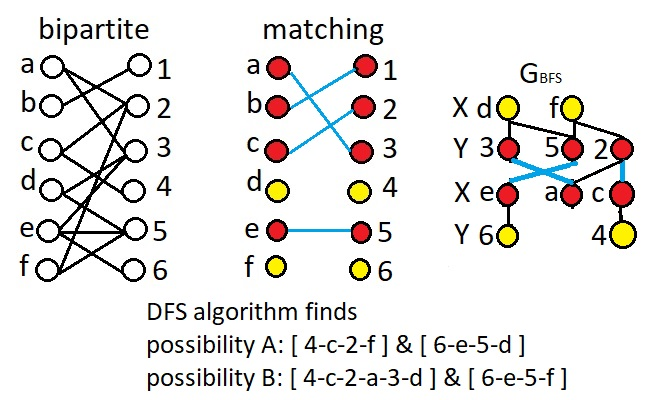
\includegraphics[scale=0.8]{hopcroftkarp_bfs.jpg}
    \caption{Finding Augmenting Paths}
\end{figure}

The graph formed by the BFS has 2 types of nodes, belonging to $X$ and belonging to $Y$. They can be imagined as stacks of layers going from top to bottom as shown in the figure. It is easy to see that the algorithm selects edges going from $X \to Y$ only when the edge is NOT present in the matching and selects edges going from $Y \to X$ only when the edge IS present in the matching.

Hence when we apply DFS from a node $v \in Y$, we are guaranteed to find a node $w \in X$ and $w \in M$ such that $(v, w) \notin M$. Similarly when we move from a node $v \in X $ and $v \in M$, we are guaranteed to find a node $w \in Y$ such that $(v, w) \in M$.

Also see that the DFS returns a path which begins and ends at nodes NOT present in the matching. Further the path contains edges alternate between $X$ and $Y$ such that all edges from $X \to Y \in M$ and all edges from $Y \to X \notin M$. Hence this path is an augmenting path.

Moreover this path is also disjoint since after using a node we immediately mark it as used. Hence it is effectively removed from the graph $G_{\mathrm{BFS}}$ and cannot be shared with any other path found by further iterations of the DFS algorithm.

\section{Time Complexity}

\subsection{Claim 1}
We make a claim that for a maximum matching $M^*$ and some matching matching $M$, the symmetric difference of $M^*$ and $M = M \Delta M^*$ has $|M^*|-|M|$ augmenting paths and these paths are vertex disjoint. 

We know that the presence of an augmenting path increases the size of $M$ by 1. So there are exactly $|M^*|-|M|$ augmenting paths. Also since the degree of each node is at max 2, the paths are vertex-disjoint.

\subsection{Claim 2}
We make a claim that there are at max $2\sqrt{N}$ iterations in the main loop. 

Notice that each iteration of the main algorithm increases the size of the matching by at least 1. Hence the shortest augmenting path is of length $\sqrt{N}$ after $\sqrt{N}$ iterations.

Since these paths will be vertex disjoint, we can say that there are at maximum $\sqrt{N}$ augmenting paths. Each of these paths increases the size of $M$ by 1 and hence $|M^*|-|M|$ is at max $\sqrt{N}$. Hence optimal matching $M^*$ will be achieved after at max $\sqrt{N}$ more iterations of the main algorithm.

\subsection{Calculating Time Complexity}
\begin{itemize}
    \item Each iteration involves BFS, DFS and augmenting $M$ with vertex disjoint paths.
    \item Both BFS and DFS take O$(|E|)$ time.
    \item Since the paths used to augment $M$ are vertex disjoint, the entire process takes O$(|V|)$ time.
    \item Hence each iteration of the main algorithm takes O$(|V|+|E|)$ = O($|E|$) time.
    \item From claim 2, we can see that there are at max O$(\sqrt{|V|})$ iterations.
\end{itemize}
So the overall time complexity is O($|E|\sqrt{|V|}$).

\section{References}
\href{https://en.wikipedia.org/wiki/Hopcroft\%E2\%80\%93Karp_algorithm}{\textcolor{blue}{Hopcroft-Karp Algorithm Wikipedia (Clickable URL)}}




\end{document}
